\chapter{Tiny Trainable Instruments}

This chapter describes the process of conceptualizing and developing this antidisciplinary thesis project, living at the interstitial spaces between the fields of \acrlong{AI}, electrical engineering, computer science, media arts, music, and pedagogy, among others.

As a reminder, all 


TODO: start this section with a vivid description of you vision for Tiny Trainable Instruments, what they do, basically how they work, and why they are significant and interesting. Without that, this feels a bit too much like a user's manual, not enough like a thesis.

In the next section I explain my personal definitions of the words that make up the title of this project.

\section{Definition of Tiny Trainable Instruments}

\subsection{Definition of tiny}

By \emph{tiny} I mean lightweight handheld instruments that you can fit in a  backpack, or take for a walk. This is inspired by my personal practice: for years I have accumulated many small tools for arts that I perform gigs with, or that I carry with me while traveling, mostly small electronic synthesizers, sound mixers, and battery-powered speakers.

Here is an example of a yellow handheld sampler with an included microphone and speaker that I enjoy for field recordings, complete with a green battery pack for portability.

\begin{figure}[ht]
  \centering
  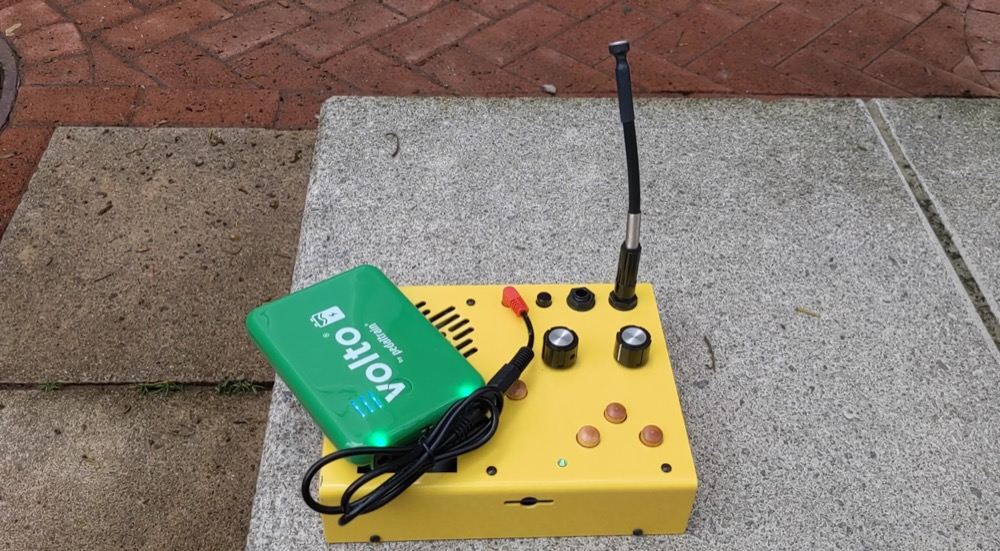
\includegraphics[width=0.75\linewidth,height=0.25\textheight,keepaspectratio]{images/critter-and-guitari-kaleidoloop-battery.jpg}
  \caption{Sampler with microphone and portable battery}
  \caption*{Picture taken by myself}
  \label{fig:critter-and-guitari-kaleidoloop-battery}
\end{figure}

\emph{Tiny} is also a nod to the emerging field and community of tiny \acrshort{ML}, including - most importantly for me - the tinyMLx professional certificate\cite{website-edx-harvardx-tinymlx-professional-certificate} offered by HarvardX, that I completed while working on this project. I have high hopes that this field can empower people to make technology that is not dependent on the cloud, big data, or centralized servers.

With that, the \emph{tiny} in \emph{Tiny Trainable Instruments} comes from them being handheld devices built on breadboards, from their being able to be powered from a generic USB power bank, and from their using tiny \acrshort{ML} processes for interpreting the data from their inputs and reacting via their outputs.

\subsection{Definition of trainable}

By \emph{trainable} I mean a device that can learn by example. This name comes from the \acrshort{ML} lexicon, where training is a process whereby an algorithm  iteratively finds the numerical values of all parameters (weights, biases) of a \acrshort{ML} model.

Training a device is particularly attractive for artists working with sensors. The Arduino microcontroller that this thesis uses has several embedded sensors, which can be used to produce huge streams of data, like this screenshot showing the output of raw data from its \acrshort{RGB} color sensor.

\begin{figure}[ht]
  \centering
  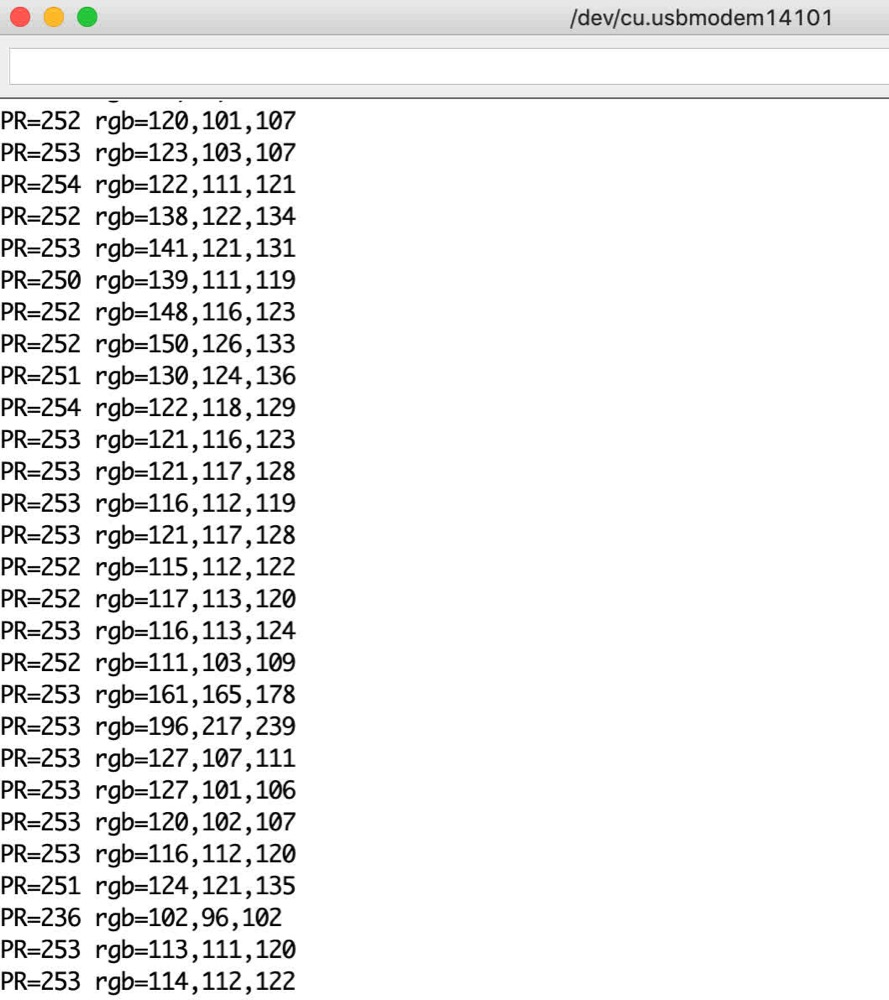
\includegraphics[width=0.75\linewidth,height=0.40\textheight,keepaspectratio]{images/arduino-data-stream.jpg}
  \caption{Data stream from embedded sensors in an Arduino microcontroller}
  \caption*{Screen capture by myself}
  \label{fig:arduino-data-stream}
\end{figure}

If we wanted to use this sensor at home to detect a red object, we would start by taking notes of the \acrshort{RGB} values of the sensor when the red object is close to it, and would then include this value as a threshold for detection on the software uploaded to the microcontroller. Since the \acrshort{RGB} sensor needs consistent lighting to work effectively, we need to be especially careful with the lighting conditions; if they change, we have to look at the stream of data to find the new value for red, and then update the code and reprogram the microcontroller.

This is a tedious process, and it inspired me to work on this thesis, so that I could help artists use \acrshort{ML} and microcontrollers to capture data, and then train a model, letting the algorithm figure out the correct answer without one having to write more code!

An educational and creative example I recommend consulting is Teachable Machine by Google \cite{website-google-teachable-machine}, a web application that allows you to use your computer's microphone and webcam to generate data, and then to train models that can detect different words, images, or body postures without having to write any line of code.

In particular, I became interested in tiny \acrshort{ML} examples that require small databases and that can be trained on-device, for the use of making an instrument whose behavior can be changed mid-performance, like guitar players do with their guitars when they change their tunings between songs. With this thesis, one can program a device that can detect an apple, and then five minutes later, an orange, and then for your last song, a grapefruit. Hat tip to Sonic Youth, a band that used to tour with more than a dozen guitars, each one of them with a different tuning; they would switch instruments between songs.

\begin{figure}[ht]
  \centering
  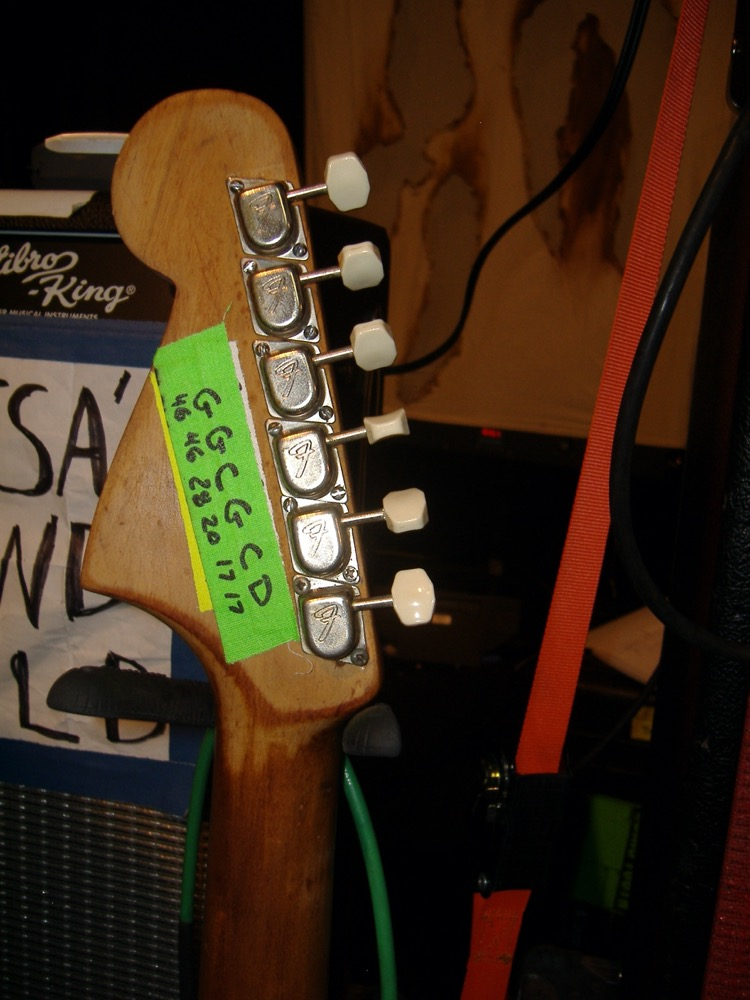
\includegraphics[width=0.75\linewidth,height=0.30\textheight,keepaspectratio]{images/sonic-youth-guitar.jpg}
  \caption{Sonic Youth guitar with custom tunings}
  \caption*{Retrieved from \cite{sonic-youth-illustrated-equipment-guide}}
  \label{fig:sonic-youth-guitar}
\end{figure}

\subsection{Definition of instruments}

By \emph{instruments} I mean devices that transduce energy across different media. Instruments receive an input, process it, and then produce an output. For musical instruments, I like to think that instruments are able to not just produce musical Western scales, but a wide spectrum of sounds encompassing the broad vocabulary of experimental electronic music and electroacoustic music.

On top of that, my personal definition of \emph{instrument} includes having freedom and liberty, not censorship. This is why I consider my bicycle to be an art instrument that transduces my pedaling input into multimedia output: adventure, sweat, and wind in my face. Also, while I am riding it, I am not subjected to the restrictions of any corporate or government playground, there are mostly no rules besides gravity, and there are no backdoors that anyone can use to track me, exploit me, or limit my speed (we have smartphones for corporate and government surveillance, but that's another story).

The liberties that \emph{instruments} make me feel are a huge contrast to the computational tools I am using for crafting this thesis. I am typing on an Apple Macbook, and even though I like its keyboard and portability, I am aware that I face restrictions: Apple wants developers to pay to be certified developers, and if I update my operating system I won't be able to run 32 bits apps anymore. This thesis is hosted on GitHub, which is a service blocked for developers in certain countries due to U.S.A. sanctions \cite{website-github-trade-controls}. I am from a country recently affected by a dictatorship and human rights violations and some of my relatives have been exiled, so I am particularly sensitive to policies that limit people's freedom of speech and computing.

This discomfort was also a catalyst for the creation of \textit{Tiny Trainable Instruments}, which are based on open source off-the-cloud microcontrollers, and nobody can censor me when I use them for arts, thus being \emph{instruments}, as gratifying as playing with my guitar and bicycle. I hope you feel that joy too while spending time with this thesis.

In this section I will explain the process and the results of each component of this thesis:

\begin{enumerate}
  \item TinyTrainable Arduino software library
  \item Code for training \acrshort{ML} with \acrshort{DIY} databases
  \item Educational material and workshop
\end{enumerate}

\section{TinyTrainable Arduino software library}

This project's main contribution is the TinyTrainable Arduino software library,  hosted at \url{https://github.com/montoyamoraga/TinyTrainable}. It allows you to create flexible multimedia instruments, where you can combine any input with any output, and it runs on the microcontroller Arduino Nano 33 BLE Sense \cite{website-materials-arduino-nano-33-ble-sense}. This microcontroller was chosen because it is currently the only Arduino supported by the Arduino TensorFlow Lite library.

\begin{figure}[ht]
  \centering
  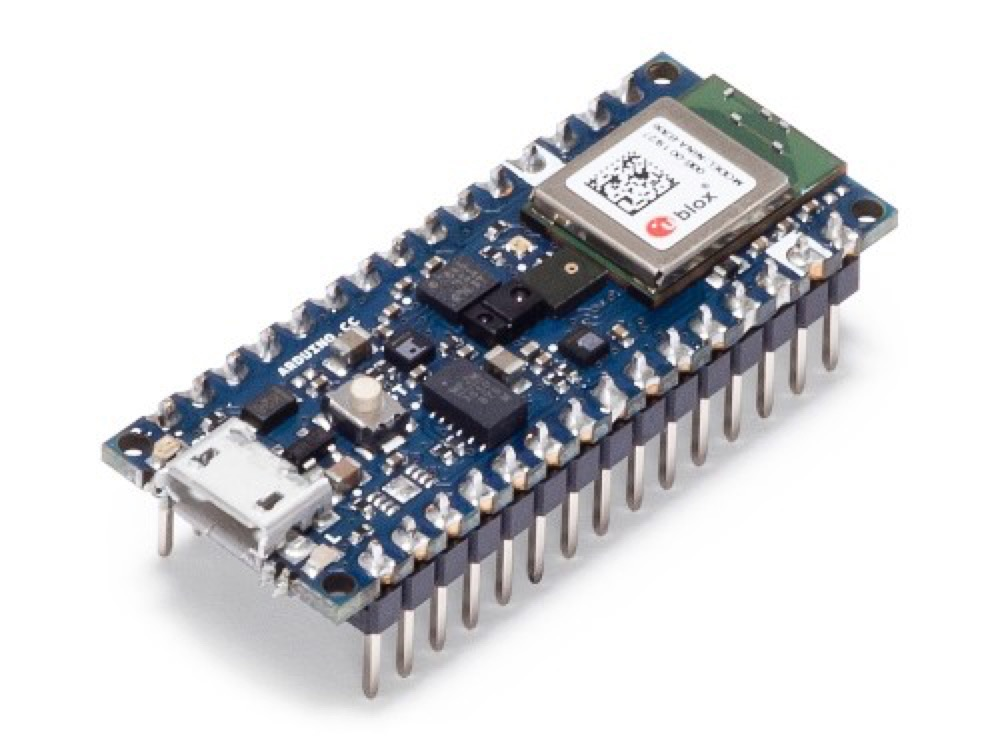
\includegraphics[width=0.75\linewidth,height=0.30\textheight,keepaspectratio]{images/materials-arduino-nano-33-ble-sense.jpg}
  \caption{Arduino Nano 33 \acrshort{BLE} Sense microcontroller with headers}
  \caption*{Retrieved from \cite{website-materials-arduino-nano-33-ble-sense}}
  \label{fig:materials-arduino-nano-33-ble-sense}
\end{figure}

The TinyTrainable library is flexible, since it allows one to combine any of the three available inputs with any of the seven possible outputs, for a total of twenty-one possibilities summarized on \ref{tiny-trainable-instruments-inputs-outputs-matrix}:

\begin{table}[ht]
    \centering
    \begin{tabular}{ | l | l | l | l | l | l | l | l |}
        \hline
        \textbf{\backslashbox{Input}{Output}}  & Buzzer & \acrshort{LED} & \acrshort{MIDI} & Printer & Screen & Serial & Servo \\
        \hline
        Color & & & & & & & \\
        \hline
        Gesture & & & & & & & \\
        \hline
        Speech & & & & & & & \\
        \hline
    \end{tabular}
    \caption{Matrix of inputs and outputs}
    \label{tiny-trainable-instruments-inputs-outputs-matrix}
\end{table}{}

For the inputs I used the embedded sensors of the Arduino microcontroller with their corresponding open source libraries, and processed the input data with two recently released open source \acrshort{ML} libraries, summarized on \ref{software-dependencies-inputs}:

\begin{table}[ht]
    \centering
    \begin{tabular}{ | l | l | l |}
        \hline
        \textbf{Input}  & \textbf{Sensor library} & \textbf{\acrshort{ML} library} \\
        \hline
        Color &  Arduino{\_}APDS9960 & Arduino{\_}KNN \\
        \hline
        Gesture & Arduino{\_}LSM9DS1 & Arduino{\_}TensorFlowLite \\
        \hline
        Speech & PDM & Arduino{\_}TensorFlowLite \\
        \hline
    \end{tabular}
    \caption{Software dependencies for inputs}
    \label{software-dependencies-inputs}
\end{table}{}

The outputs are actuators that  rely on extra hardware, and in some cases, external libraries, which are summarized in \ref{software-dependencies-outputs}.

\begin{table}[ht]
    \centering
    \begin{tabular}{ | l | l | }
        \hline
        \textbf{Output}  & \textbf{Actuator library} \\
        \hline
        Buzzer & - \\
        \hline
        \acrshort{LED} & - \\
        \hline
        \acrshort{MIDI} & - \\
        \hline
        Printer & Adafruit Thermal Printer Library\\
        \hline
        Screen & Adafruit{\_}SSD1306\\ 
        \hline
        Serial & - \\
        \hline
        Servo & Servo\\
        \hline
    \end{tabular}
    \caption{Software dependencies for outputs}
    \label{software-dependencies-outputs}
\end{table}{}

The behavior of the TinyTrainable library is already designed, and is explained in this chapter. The software implementation is in flux, and I do my best to publish new releases with notes on how the library has changed over time, including bug fixes, clearer language for the examples, and different ways of interfacing with the methods and variables of the TinyTrainable library.

This library is a repository hosted on GitHub, to foster collaboration via \glspl{issue} and \glspl{pull-request}. Each \glspl{commit} is annotated and commented, in order to show people the whole process and effort involved in writing this thesis project.

\subsection{Repository structure}

The TinyTrainable library is a repository hosted at \url{https://github.com/montoyamoraga/TinyTrainable}, where one can review all the history and \glspl{commit}, to see how the whole library or each file has evolved over time.

The structure of the folders follows two simultaneous specifications: it includes the necessary file and folder names for being packaged and indexed as an Arduino Library, and on top of that it complies with GitHub guidelines for licensing libraries, and for automatic workflows for code testing.

The source code of the library is written in C++ and is located in the src/ folder. The examples live in the examples/ folder, and are written in the Arduino language. The examples are divided into four folders: one for each input, and one extra for checking the wiring of each output. In the assets/ folder, I included some C++ files with trained models for the examples.

\subsection{Installation}

The library can be downloaded from the Releases section of the repository at  \url{https://github.com/montoyamoraga/TinyTrainable/releases}, where you also have access to the complete history of releases over time. To install it, you need to uncompress the .zip into a folder, and then make it discoverable by the Arduino \acrfull{IDE}.

Since that method is not automatic and could be prone to errors, I made the effort to publish the TinyTrainable library, by complying with the latest Arduino Library Manager specifications, detailed on their repository \url{https://github.com/arduino/library-registry/}. With that, from the Arduino \acrshort{IDE} you can open their Library Manager and do a 1-click installation of the library, or as an alternative use arduino-cli, the Arduino command line tool on your terminal.

\subsection{Hardware basics}

The TinyTrainable library at its current iteration has only one strict hardware requirement: it only runs on the Arduino Nano 33 \acrshort{BLE} Sense, a microcontroller released in 2019. For powering it you need a generic micro USB cable, which can also be used to upload code to it from a computer running the Arduino IDE.

\begin{figure}[ht]
  \centering
  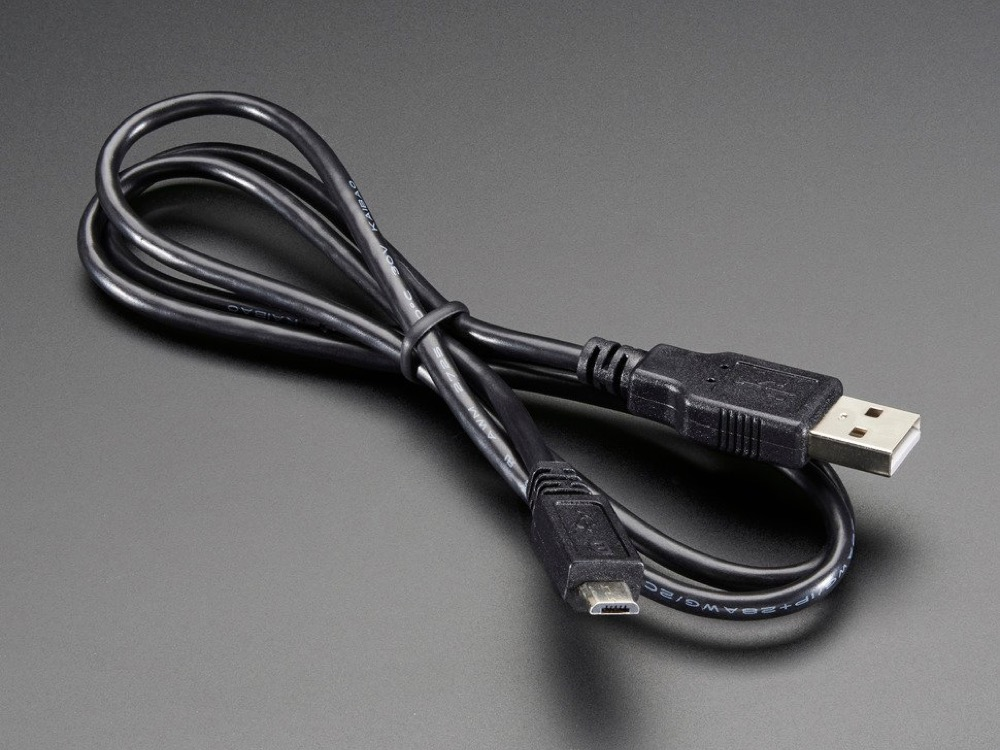
\includegraphics[width=0.75\linewidth,height=0.25\textheight,keepaspectratio]{images/materials-adafruit-micro-usb-cable.jpg}
  \caption{Micro USB cable}
  \caption*{Retrieved from \cite{website-materials-adafruit-micro-usb-cable}}
  \label{fig:materials-adafruit-usb-cable}
\end{figure}

To build a Tiny Trainable Instrument, you also need a breadboard, where you can place the Arduino microcontroller, and some jumper wires to connect it to one of the many possible output devices that I will describe soon.

\begin{figure}[ht]
  \centering
  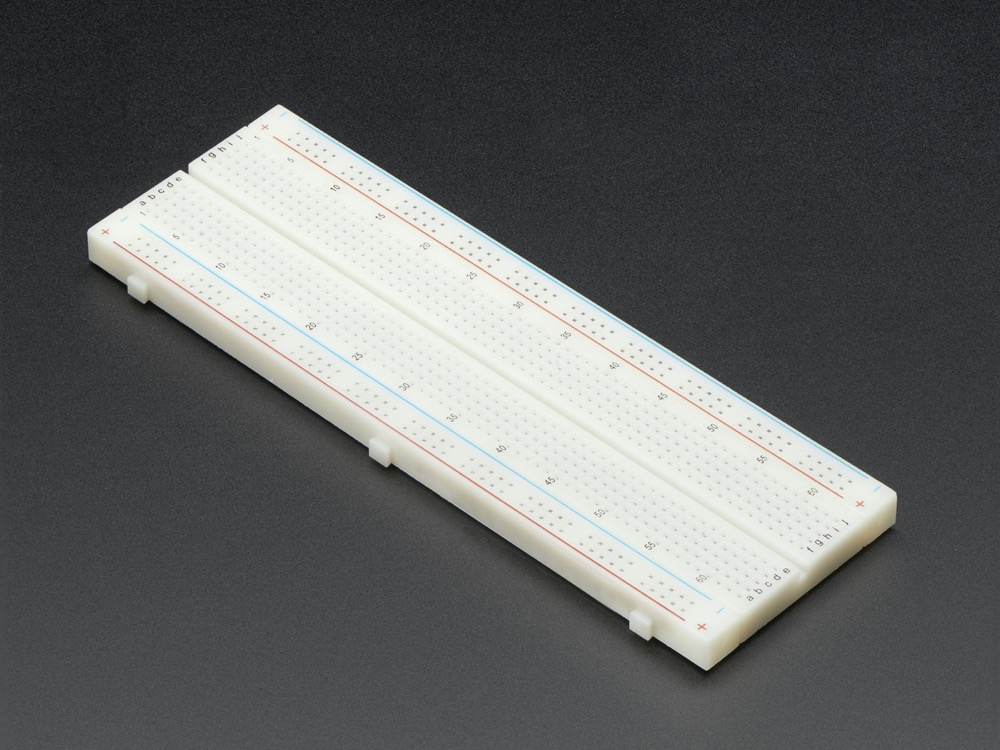
\includegraphics[width=0.75\linewidth,height=0.25\textheight,keepaspectratio]{images/materials-adafruit-breadboard.jpg}
  \caption{Breadboard}
  \caption*{Retrieved from \cite{website-materials-adafruit-breadboard}}
  \label{fig:materials-adafruit-breadboard}
\end{figure}

\begin{figure}[ht]
  \centering
  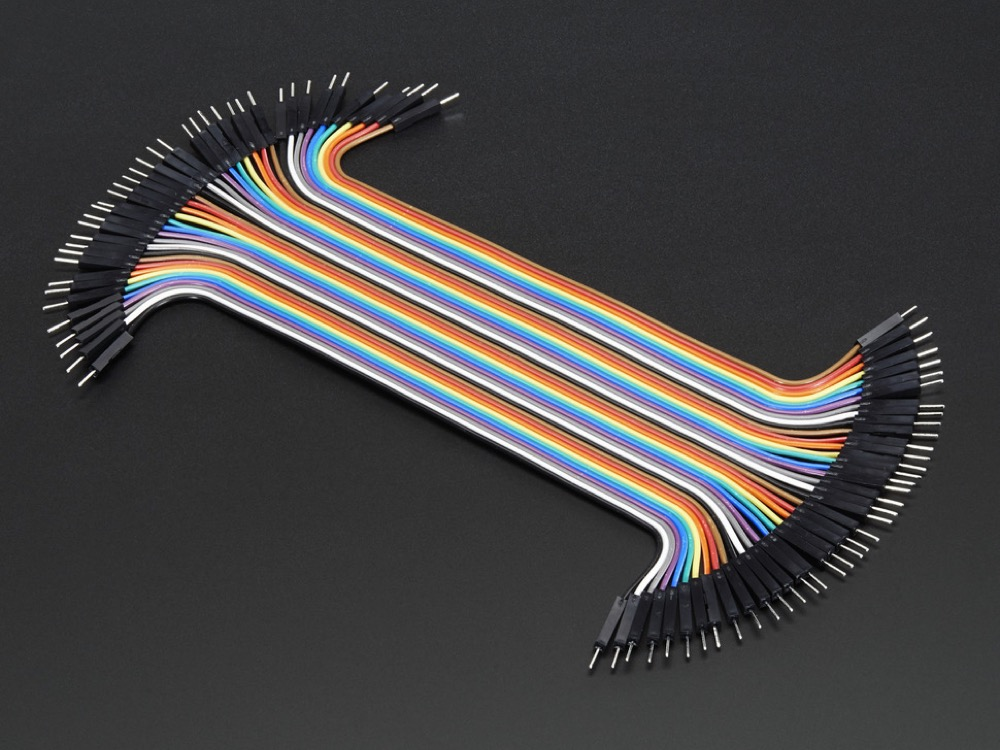
\includegraphics[width=0.75\linewidth,height=0.25\textheight,keepaspectratio]{images/materials-adafruit-jumper-wires.jpg}
  \caption{Jumper wires}
  \caption*{Retrieved from \cite{website-materials-adafruit-jumper-wires}}
  \label{fig:materials-adafruit-jumper-wires}
\end{figure}

\subsection{Inputs}

As I mentioned before, for the inputs no extra wiring is needed, since we are using the embedded sensors of the Arduino microcontroller to detect the three possible inputs: color, gesture, and speech. These inputs were designed to foster different behaviors with the library, which are detailed in the following sections.

I decided that each input would be able to detect only three different categories, because I thought that more categories would make the instruments more cumbersome to train, needing larger databases, and longer training times. Hopefully in the future I can adapt the TinyTrainable library to make this a variable number of categories it can classify, but for now this is hardcoded in the library. Nonetheless, if you want to use the library for your own project with a different number of categories, since the library is open source and documented, it should be easy to adapt it to your needs.

\subsection{Color input}

The color input allows artists to build Tiny Trainable Instruments that can detect three different colors of objects near the microcontroller. I recommend that this is the first input that people try, since it is the easiest and fastest of the other inputs to learn and use. It is based on the examples included with the Arduino{\_}KNN library \cite{repository-arduino-knn}.

When detecting color, the library acts as a wrapper of the Arduino{\_}APDS9960 library \cite{repository-arduino-APDS9960}, needed to access the data of the embedded distance and color sensor of the microcontroller. Both of these sensors are used together, so that the instrument can detect nearby objects, and when they are close to the microcontroller, it reads a one pixel \acrshort{RGB} value, detecting how red, how green, and how blue any object is.

This \acrshort{RGB} data is stored in the microcontroller, to build a database that then is used to train a \acrshort{ML} algorithm, in particular a \acrfull{k-NN}, implemented with the Arduino{\_}KNN library. After the algorithm is trained, the instrument is able to detect between the three different colors.

The main difference between this input and the other ones, is that both the data capture and the model training happen on the device, and it is not persistent: every time the Arduino microcontroller is turned on it needs to be trained again. This behavior has the upside of making the data input and the trained model never leave your microcontroller, for enhanced privacy. The downside is that you cannot preserve the data or the model, which are erased when the microcontroller is disconnected from power.

\subsection{Gesture input}

The gesture input allows artists to build Tiny Trainable instruments that can detect three different motion gestures, by moving the microcontroller in space. It is based on the Magic Wand example of the Arduino TensorFlow Lite library \cite{repository-tensorflow-tflite-micro-magic-wand}.

\begin{figure}[ht]
  \centering
  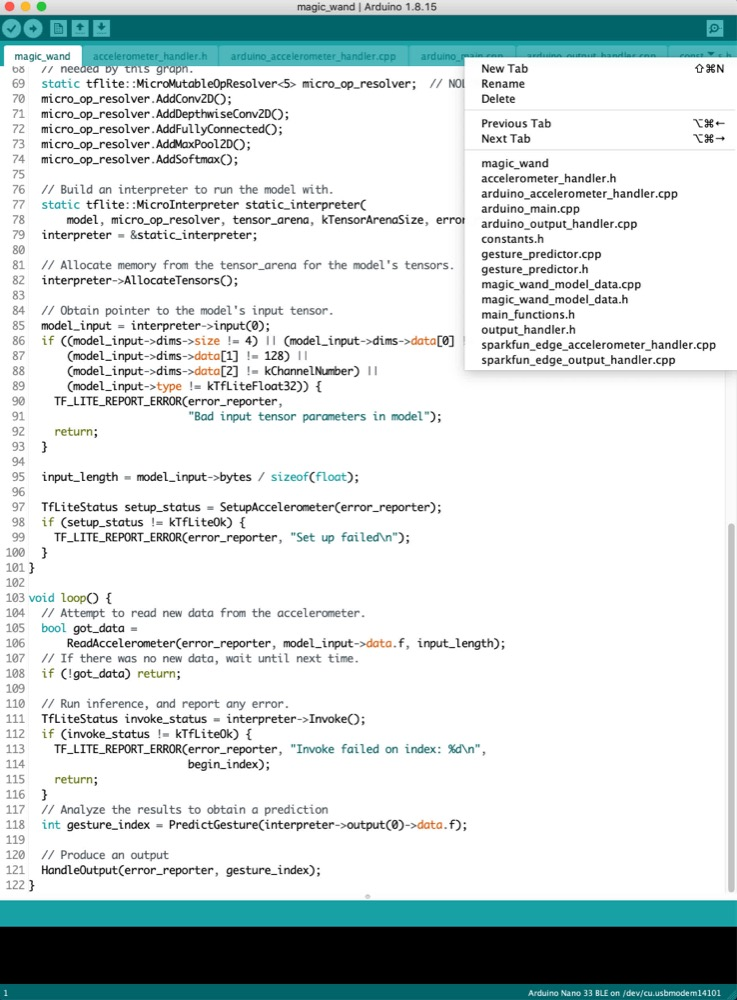
\includegraphics[width=0.75\linewidth,height=0.40\textheight,keepaspectratio]{images/arduino-tensorflow-lite-magic-wand.jpg}
  \caption{Magic wand example}
  \caption*{Screen capture by myself}
  \label{fig:arduino-tensorflow-lite-magic-wand}
\end{figure}

This Magic Wand example is able to detect gestures, and print the result over a serial port. It is made up of several files, and to make modifications you have to replace code in various of these files. The TinyTrainable library acts as a wrapper for this complexity, only exposing to the user some variables and methods for setting up the instrument.

The equivalent example in the TinyTrainable library that has the same functionality as Magic Wand is called gestures{\_}serial. Currently it is only 36 lines of code, most of them comments or space, plus a file with the trained model. The TinyTrainable library also expands the original functionality of outputting messages over serial port, to include the other six outputs supported.

When detecting gestures, the TinyTrainable library acts as a wrapper of the Arduino{\_}LSM9DS1 library \cite{repository-arduino-LSM9DS1} , needed to access the data of the embedded \acrfull{IMU}. The library includes an Arduino sketch to capture the data of the three gestures we want to recognize, which then needs to be saved on a computer. These files with the database are imported in a Jupyter notebook to train the \acrshort{ML} model with Google TensorFlow. The trained model is then used with the TinyTrainable library and uploaded to the Arduino microcontroller to detect the three different gestures.

Even though for both the color input and the gesture input we use the Arduino to capture the data, for the gesture input we do need a computer to process the data; the drawback is that we still need a computer for training the model. A positive aspect is that the training is persistent: the Arduino microcontroller only needs to be trained once for the same database, and remembers the model every time it is turned on, unlike the color input which forgets the trained model.

A contribution of this thesis is that it expands existing examples that rely on the cloud, in particular the freemium service Google Colaboratory \cite{website-google-colab} (or Colab for short). Training on the cloud has some advantages; for example, in this case the Google Colab resources are faster than training on my own and most computers, but I think this comes at the expense of losing privacy.

These gesture databases we are creating do not include compromising information, or make you identifiable for governments or corporations, like your fingerprints or your DNA. Because of these low-stakes, I don't discourage people from using Google Colab with this thesis, but I do want to stress that we can circumvent these corporate systems. For this reason, a contribution of my thesis is that I am including code and strategies for people to be able to train the models on their own computers, in a more private way.

\subsection{Speech input}

The speech input allows artists to build Tiny Trainable instruments that can detect three different sounds or utterances, by emitting sound next to the microcontroller.  It is based on the Micro Speech example of the Arduino TensorFlow Lite library.

\begin{figure}[ht]
  \centering
  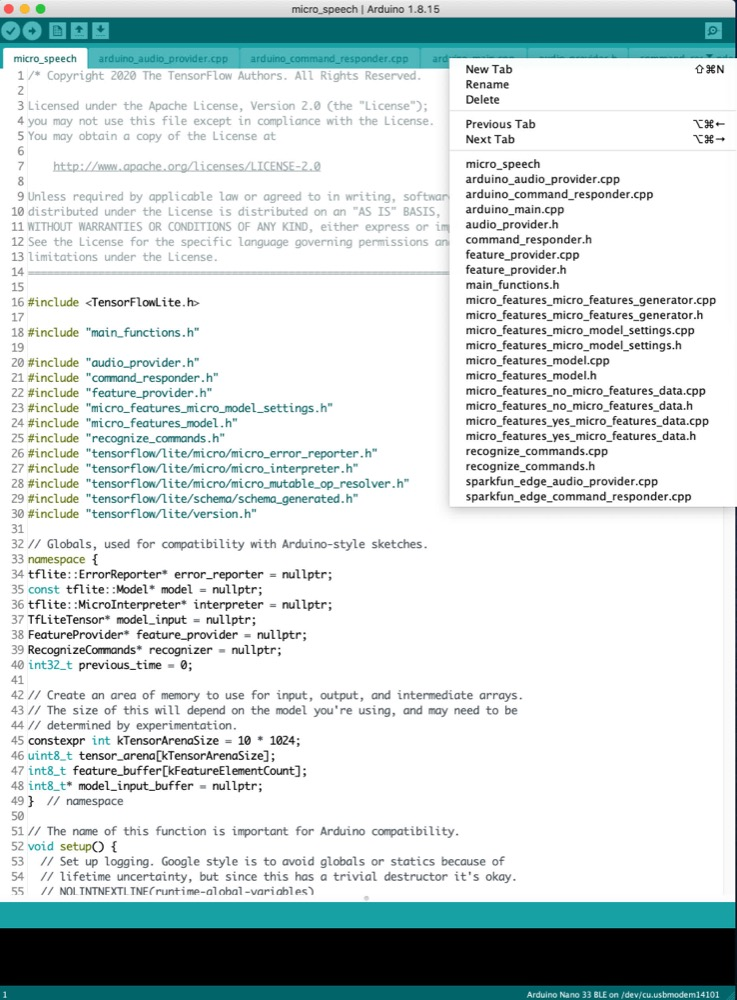
\includegraphics[width=0.75\linewidth,height=0.40\textheight,keepaspectratio]{images/arduino-tensorflow-lite-micro-speech.jpg}
  \caption{Micro speech example}
  \caption*{Screen capture by myself}
  \label{fig:arduino-tensorflow-lite-micro-speech}
\end{figure}

This Micro Speech example is able to detect speech utterances, and print the result over a serial port. It is made up of several files, and to make modifications you have to replace code in various of these files. The TinyTrainable library acts as a wrapper for this complexity, only exposing to the user some variables and methods for setting up the instrument.

The equivalent example on the TinyTrainable library that has the same functionality as Micro Speech is called speech{\_}serial. Currently it is only 34 lines of code, most of them comments or space, plus a file with the trained model. The TinyTrainable library also expands the original functionality of outputting messages over serial port, to include the other six outputs supported.

When detecting speech, the library acts as a wrapper of the PDM library \cite{repository-arduino-PDM}, used to access the \acrfull{PDM} data of the embedded microphone. This input is the only one where we are not using the microcontroller to capture the data: the documentation includes instructions for building your own database with the microphone in your computer, in order to capture the data of the three different words we want to recognize. 

In a similar fashion as the gesture input, the database files are then imported in a Jupyter notebook to train the \acrshort{ML} model with Google TensorFlow. The trained model is then used with the TinyTrainable library and uploaded to the Arduino microcontroller to detect the three different words.

The speech input is the most complex and time-consuming one to implement, and we need a computer for both capturing the data and training the model. A positive aspect is that just like the gesture input, the training is persistent, the Arduino microcontroller only needs to be trained once for the same database, and remembers the model every time it is turned on, unlike the color input which forgets the trained model.

Just like the gesture input, the speech input can be trained either on the cloud using Google Colab, or can be trained on your machine. Because of its complexity, I do advise that the time difference is significant: on my Macbook the model took between one and two days to train, in comparison with the gesture model which takes around two hours on my machine.

The speech database we built is the most compromising one, since it is identifiable, and it could even be used for cloning our voice with deepfake techniques. So this is the one I encourage people to be more mindful about when publishing their custom databases.

\subsection{Outputs}

The seven possible outputs of the TinyTrainable library were chosen to showcase many artistic mediums, with the hope that this library can be incorporated into the practice of artists working with light, visuals, sound, sculpture, dance, and poetry, among others.

The TinyTrainable library includes four examples for each one of the seven outputs: one for checking that the wiring is correct on the breadboard, and combinations with each one of the three inputs. Each example is an homage to the classic \emph{hello world} examples of computer science education; that is, they are introductory building blocks, intended to teach artists the basics of each output so then they can continue on their own.

All the materials for the outputs are illustrated by the corresponding image of the product page on the website Adafruit, which I recommend for beginners and artists interested in building their own Tiny Trainable Instruments.

\subsection{Buzzer output}

The buzzer is a device that can vibrate and that emits sound. The TinyTrainable library allows you to output a different sound for each of the three different input classifications, by controlling two fundamentals of the sound: frequency and duration.

\begin{figure}[ht]
  \centering
  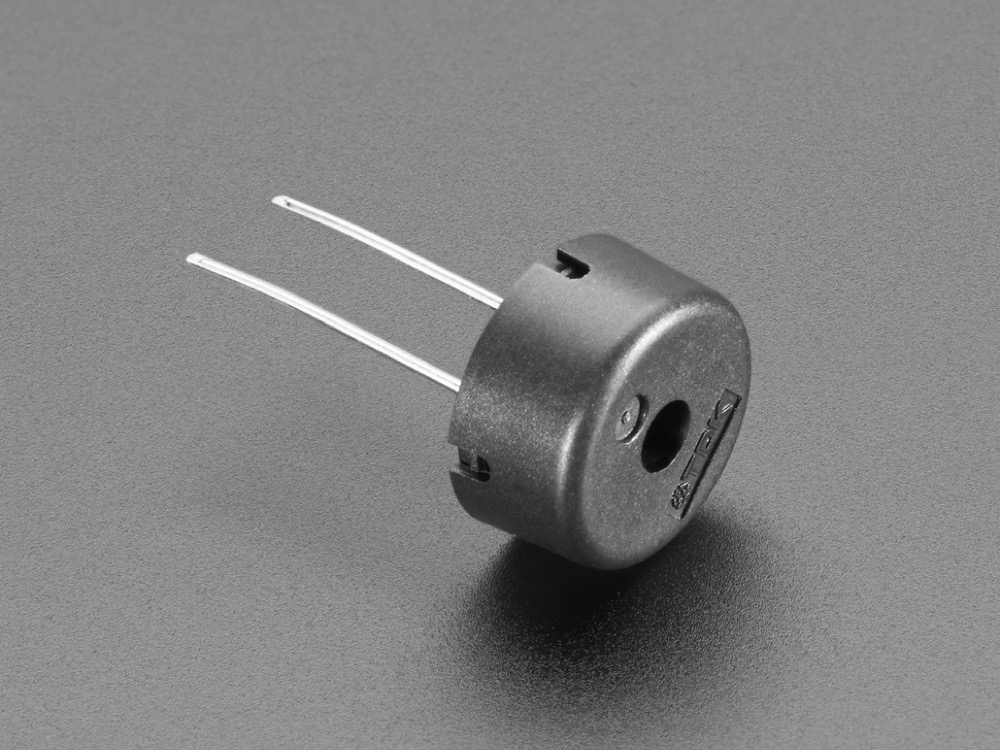
\includegraphics[width=0.75\linewidth,height=0.25\textheight,keepaspectratio]{images/materials-adafruit-buzzer.jpg}
  \caption{Buzzer}
  \caption*{Retrieved from \cite{website-materials-adafruit-buzzer}}
  \label{fig:materials-adafruit-buzzer}
\end{figure}

I included support for the buzzer because of its low cost and low fidelity sound. I think these specifications make a great contrast with the high complexity of the technology involved in doing tiny \acrshort{ML}. I consider Tiny Trainable Instruments with buzzer output to be cutting-edge technology driving a cheap buzzing sound. This is an inviting and playful combination that I also want to convey in the other outputs of this project.

This output requires no additional libraries; the Arduino microcontroller by itself is able to generate the \acrfull{PWM} output required to drive the buzzer.

\subsection{LED output}

The \acrfull{LED} is a cheap and fundamental element for making art with lights. The TinyTrainable library allows you to toggle on and off three different LEDs, depending on which of the three possible inputs was detected by the \acrshort{ML} algorithm.

\begin{figure}[ht]
  \centering
  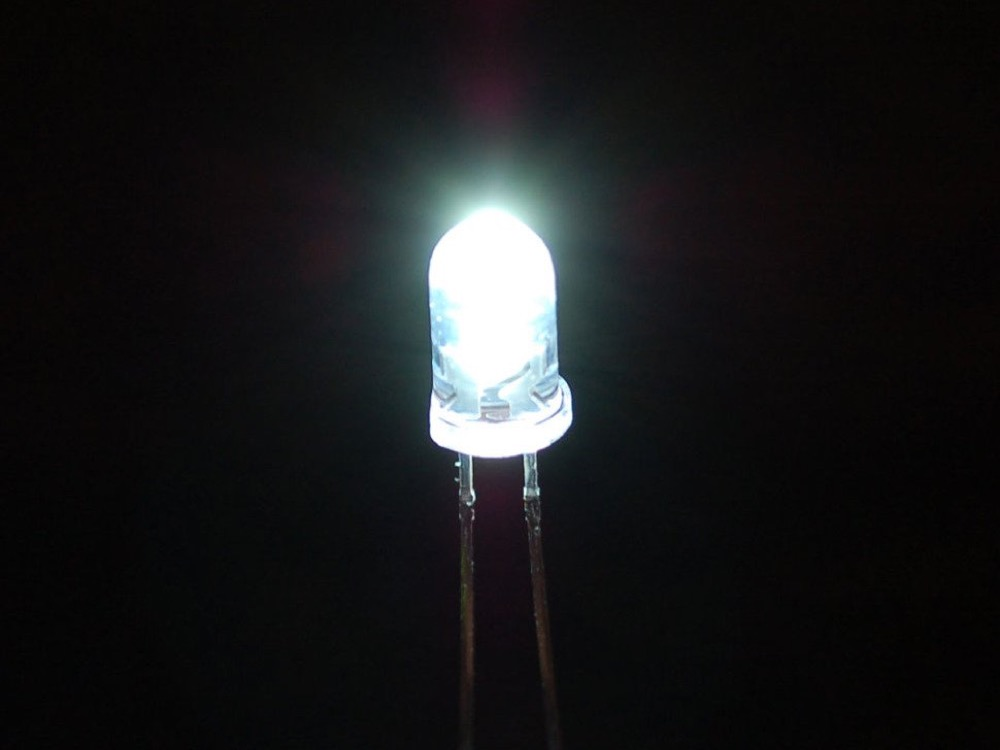
\includegraphics[width=0.75\linewidth,height=0.25\textheight,keepaspectratio]{images/materials-adafruit-led.jpg}
  \caption{LED}
  \caption*{Retrieved from \cite{website-materials-adafruit-led}}
  \label{fig:materials-adafruit-led}
\end{figure}

This output requires no additional libraries, the Arduino microcontroller by itself is able to provide enough power to light up most hobby LEDs.

\subsection{MIDI output}

\acrfull{MIDI} is a protocol invented in the 1980s to allow musical instruments to be interconnected and share information, including musical notes, control parameters, and timing. Traditionally, MIDI instruments have a 5 pin  \acrshort{DIN} connector, (from the German \acrlong{DIN}), like the one pictured here for use on a breadboard.

\begin{figure}[ht]
  \centering
  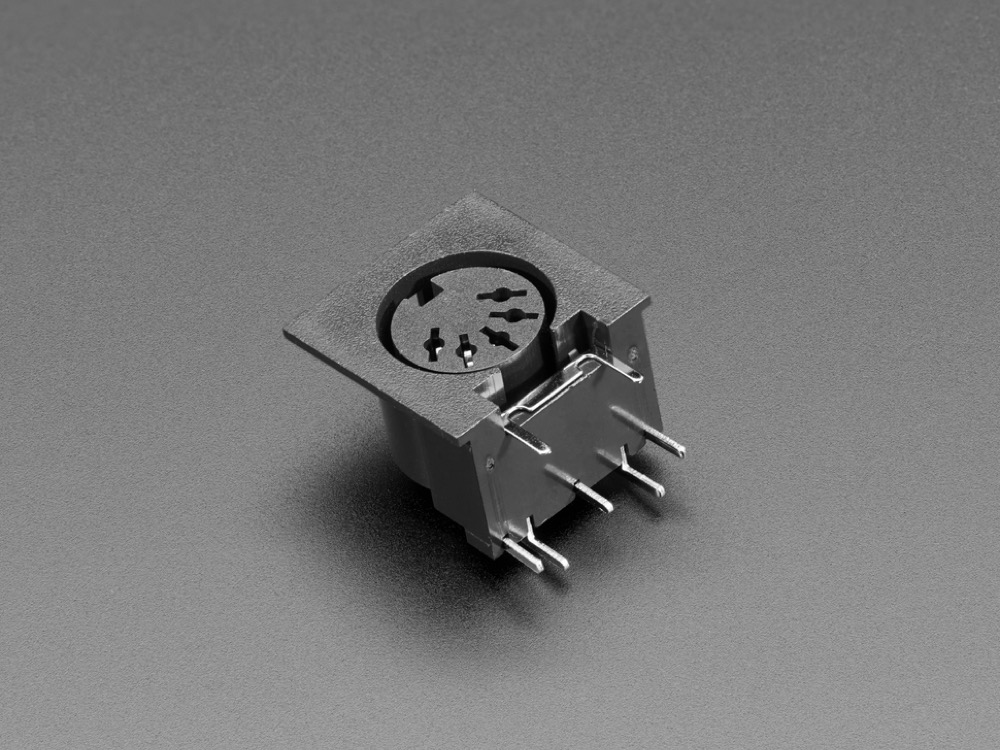
\includegraphics[width=0.75\linewidth,height=0.25\textheight,keepaspectratio]{images/materials-adafruit-midi-jack.jpg}
  \caption{MIDI DIN connector}
  \caption*{Retrieved from \cite{website-materials-adafruit-midi-jack}}
  \label{fig:materials-adafruit-midi-jack}
\end{figure}

MIDI can be used for transmitting all sorts of data, and thesis examples show how to use MIDI to control different aspects of MIDI-enabled instruments, including synthesizers and drum machines. As a bonus, I wrote examples to interface with three synthesizers from the volca series by Korg: volca bass (analog bass machine), volca beats (drum machine), and volca keys (polyphonic synthesizer). I picked these synthesizers to have both melodic and percussive musical elements, because of their huge popularity, their relatively low price of 150.00 USD, their extensive MIDI capabilities, and because I am a huge fan of the instrument designs by Tatsuya Takahashi \cite{website-tatsuya-takahashi}.

This output requires no additional libraries, since the Arduino microcontroller by itself is able to communicate via serial protocol, and the MIDI protocol is a subset of serial, at a particular \gls{baud} rate.

\subsection{Printer output}

I used to associate printing with expensive toners and ink cartridges, and mostly with frustration. This radically changed when I took a physical computing class, where I learned about thermal printers and how I could use Arduino microcontrollers to drive them! I find these thermal printers amazing because they are mostly a one-time investment and they don't need anything besides paper and power, so I have used them for interactive art installations since then. That is why I decided to include support for them on this project.

The thermal printer kit I recommend on the bill of materials is around 60.00 USD, and includes the power supply and paper roll. I picked this one because it is sold and supported by Adafruit, and I am a huge fan of their software libraries and tutorials. 

\begin{figure}[ht]
  \centering
  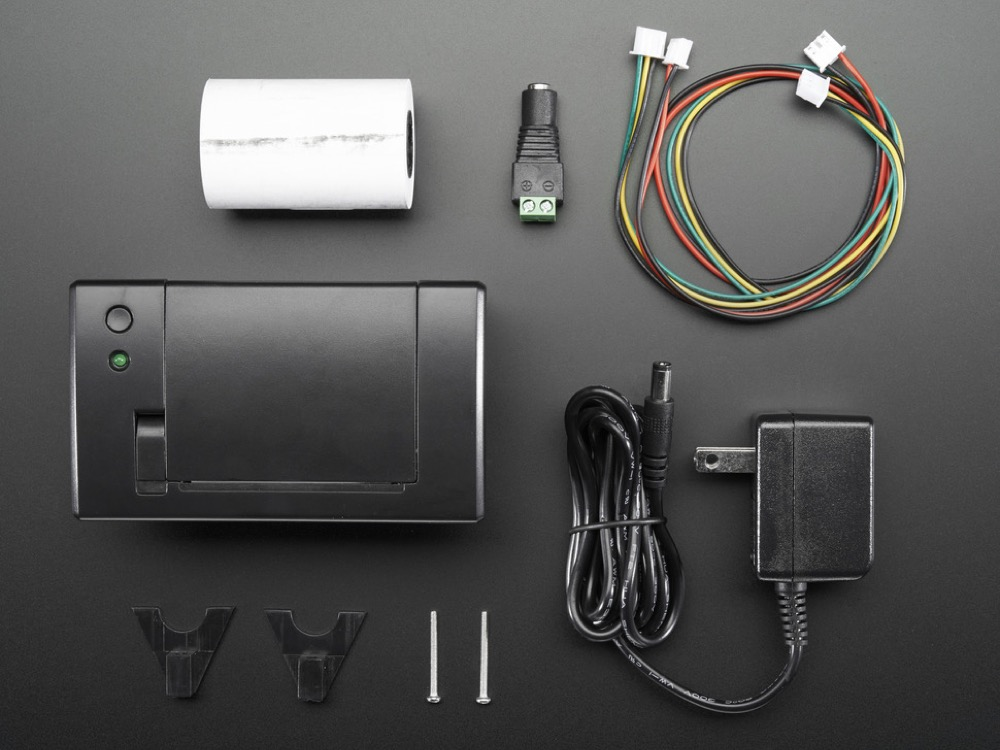
\includegraphics[width=0.75\linewidth,height=0.25\textheight,keepaspectratio]{images/materials-adafruit-thermal-printer.jpg}
  \caption{Thermal printer kit}
  \caption*{Retrieved from \cite{website-materials-adafruit-thermal-printer}}
  \label{fig:materials-adafruit-thermal-printer}
\end{figure}

With this output, you can create a Tiny Trainable Instrument that can print different texts and in various fonts and formatting, depending on the classification of the input. I hope this inspires a new generation of computer poets and interactive literature!

This output requires one additional library, the Adafruit Thermal Printer library, which is open source and includes several examples for expanding the functionality of it. If you want to use an alternative hardware or software for thermal printing, I recommend you modify the TinyTrainable library, and include any other additional software you want.

\subsection{Screen output}

In contrast to the static nature of the output of the thermal printer, which prints a fixed message on a piece of paper, I included support for using a screen for dynamic messages on a surface. 

\begin{figure}[ht]
  \centering
  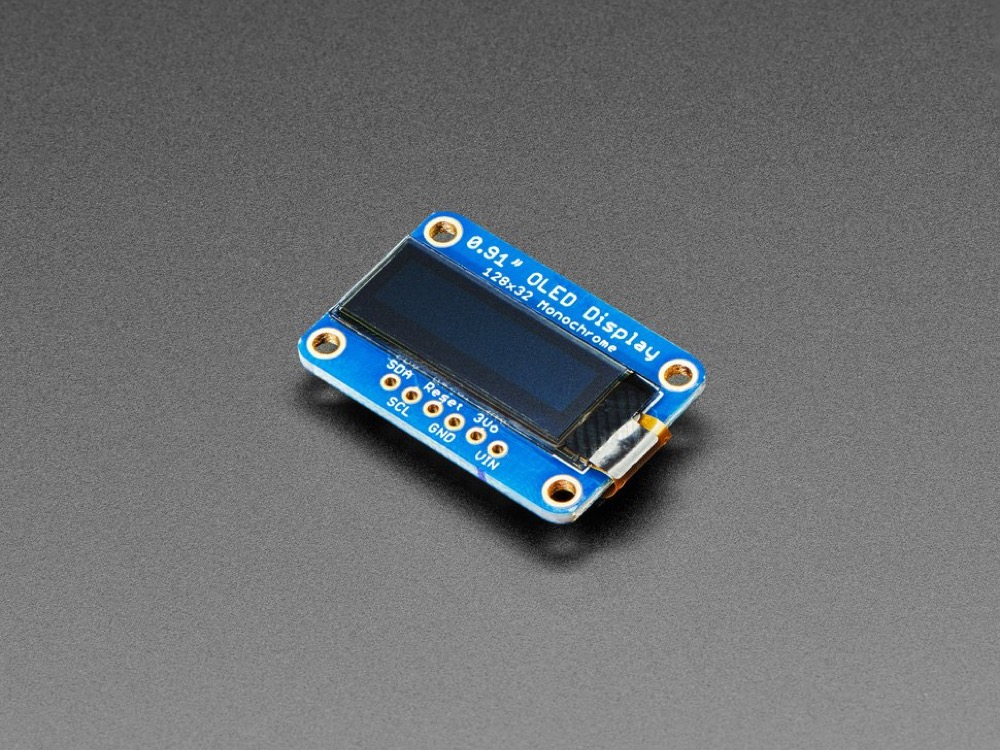
\includegraphics[width=0.75\linewidth,height=0.25\textheight,keepaspectratio]{images/materials-adafruit-screen.jpg}
  \caption{Screen}
  \caption*{Retrieved from \cite{website-materials-adafruit-screen}}
  \label{fig:materials-adafruit-screen}
\end{figure}

This output requires 1 additional library, the Adafruit{\_}SSD1306 library (and its own dependencies), for the particular screen I recommend on the bill of materials. The same vendor Adafruit offers many alternatives in different sizes, technologies, and color support. I encourage people to use different screens from different vendors, and \gls{fork} and adapt the TinyTrainable library to accomplish it.

\subsection{Serial output}

This output uses the same USB cable we mentioned earlier, for delivering the power and uploading code to the Arduino microcontroller. We can use the same cable to send messages over the serial protocol, and receive them on the Arduino IDE, or in any other software that reads from the serial port.
\begin{figure}[ht]

  \centering
  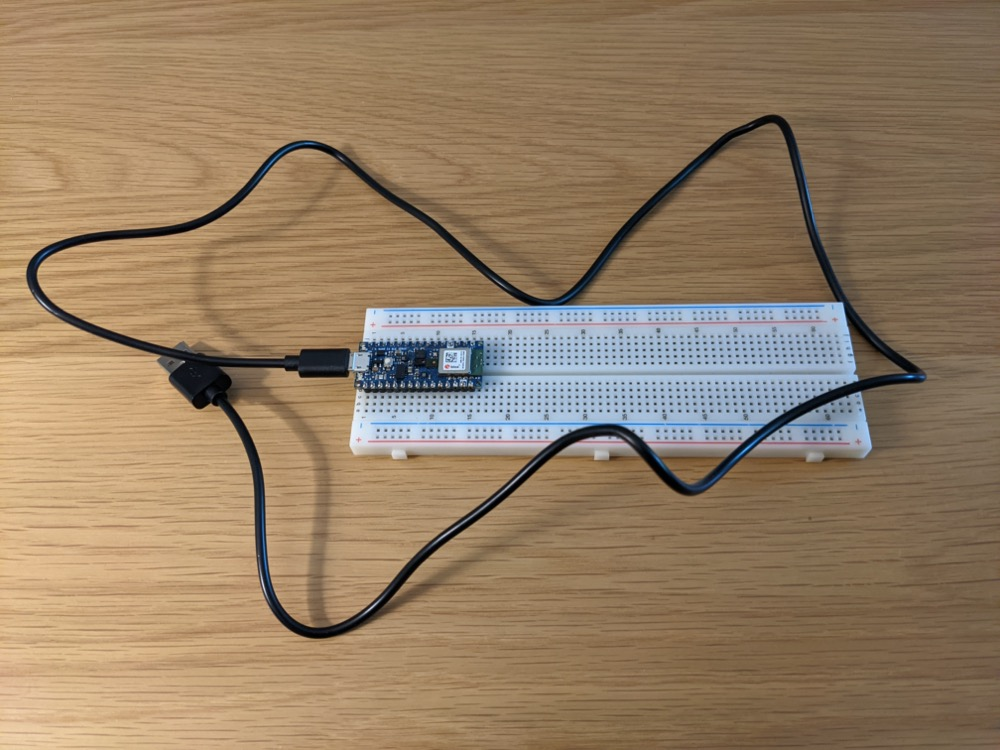
\includegraphics[width=0.75\linewidth,height=0.25\textheight,keepaspectratio]{images/output-serial.jpg}
  \caption{Tiny Trainable Instrument with serial output}
  \caption*{Picture taken by myself}
  \label{fig:output-serial}
\end{figure}

This output is useful for proofs of concept, for quick testing of the input classification before wiring a more complex output, and also for doing low-level communication with other serial software on your computer. 

This output requires no additional libraries, since the Arduino microcontroller by itself is able to communicate via serial protocol, and the MIDI protocol is a subset of serial, at a particular \gls{baud} rate.

\subsection{Servo output}

This final output is one of the cheapest ones, along with the buzzer, and that is why both were included in the thesis workshop. This is another example taken from the tradition of learning how to use servo motors in physical computing classes when learning how to program Arduino microcontrollers. That is why I included support for them in the library.

\begin{figure}[ht]
  \centering
  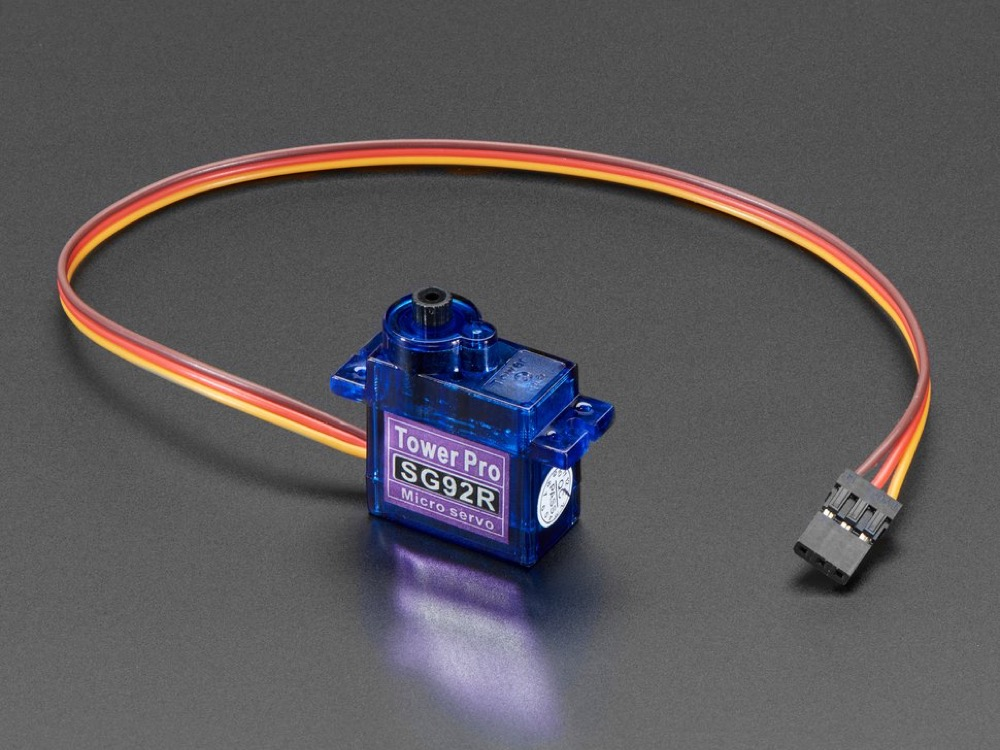
\includegraphics[width=0.75\linewidth,height=0.25\textheight,keepaspectratio]{images/materials-adafruit-servo.jpg}
  \caption{Micro servo motor}
  \caption*{Retrieved from \cite{website-materials-adafruit-servo}}
  \label{fig:materials-adafruit-servo}
\end{figure}

I see the servo motor as a very versatile output, which can be thought of as a generator of movement. So our Tiny Trainable Instrument can dance in space, or point at different places. For this library, I programmed support for moving the servo at different tempos, even with some random noise for hiccupy movement, so that the servo motor can be thought of as a robotic arm for drumming or tapping on different surfaces for music. In this image, you can see an example of this with some tape and wire for extending the arm of the servo motor.

This output requires no additional libraries. The Arduino microcontroller by itself is able to generate the \acrfull{PWM} output required to drive the servo.

\begin{figure}[ht]
  \centering
  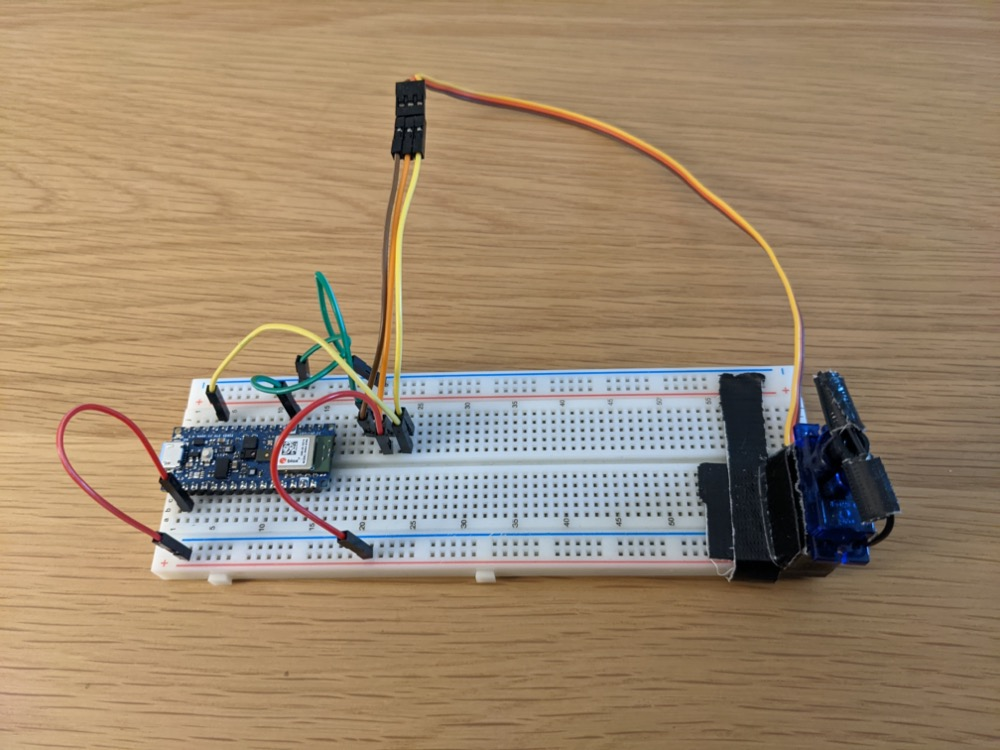
\includegraphics[width=0.75\linewidth,height=0.25\textheight,keepaspectratio]{images/output-servo.jpg}
  \caption{Tiny Trainable Instrument with servo output}
  \caption*{Picture taken by myself}
  \label{fig:output-servo}
\end{figure}

\section{Code to build databases and train ML models}

One of the biggest challenges I have encountered when working with \acrshort{ML} is to find a suitable database, that I am comfortable to work with, and that I know how to use. Often, the solution to my artistic project is building my own databases, which I have done in the past by scraping the web, or doing very tedious manual work. I do these experiments on my computer and do not publish them because I don't want to infringe on anyone's copyright.

This project does not include techniques for web scraping, since I don't want anyone to run into legal trouble, and also because I enjoyed using the Arduino microcontroller and my computer in the privacy of my room, to build the necessary databases for gesture and speech recognition, and I want to share that with artists.

In the repository that holds this thesis document, available at \url{https://github.com/montoyamoraga/tiny-trainable-instruments}, I included a folder called \emph{notebooks/}, with Jupyter notebooks written in Python 3 and using the Google TensorFlow library for training.

\section{Educational material and workshop}

In this thesis my aim is to acknowledge all the steps, dependencies, and labor needed to create the project. It has been built in small increments, which have been saved and published in the repositories that make up this project, because there is a great educational and scholarly value in documenting and reading the history of a project. This is also a way to give back to the community of artists who generously share not only the output of their work, but also their process and their tools.

This educational aspect is present throughout the included documentation: the source code is commented, there are README files for helping navigate each repository and their folders, the TinyTrainable library includes examples with each section commented and explained, and the library complies with the Doxygen standard for generating automatic documentation.

I also designed, wrote, and taught a remote workshop for beginners with the TinyTrainable library, which is explained in detail in the next chapter.

\section{Design principles}

Here is a summary of the main design principles I followed when making decisions and building this thesis project.

\subsection{Affordable}

The software library is virtually free, and it can be downloaded from the internet at no monetary cost; only bandwidth and time and hard drive costs.

The materials picked were the cheapest ones I could think of, and they are often used in similar educational contexts because they can be reusable and are forgiving to mistakes. The microcontroller is a one-time investment, and the outputs range from 2.00 USD to 60.00 USD. 

The materials for the workshop for building Tiny Trainable Instruments with buzzer, serial, and servo outputs had a cost of only 60.00 USD, including shipping.

\subsection{Open}

All examples included with this library were written with the aim of showing the fundamentals of how to build the instruments and different \acrshort{ML}-enabled manipulation of multimedia material, so that people could build on top of it and make it their own, by changing the values of variables and adding more functionalities.

\subsection{Remixable}

All the process and the code is open, and I wish that the TinyTrainable library can be used as a dependency on other people's projects. I also hope that people modify this project and make it their own, building their own spin-offs. 

\subsection{Private}

A huge emphasis I wanted to stress is to make people feel safe while handling the data. Maybe nowadays we are used to being surrounded by surveillance cameras when we are in public, or even at our homes with devices that listen to us and are connected to the cloud. I hope that this thesis can provide a computational experience that feels safe, respects your privacy, and makes you critical and aware of the issues of modern industrial machine learning applications.

\section{Development}

This thesis has been developed in collaboration with MIT undergrad researchers Peter Tone and Maxwell Wang, and funded by the MIT UROP office and the MIT Media Lab. Peter Tone helped with research in data structures, library writing, and programming different sections of the library, from the most experimental features to the most polished ones, and also helped with the design of the user-facing methods and variables. Maxwell Wang helped with proofreading the code, making sure the language of the examples and documentation were appropriate for beginners, and helped with the planning and conceptualization of the workshop. 

This collaboration was remote, and made possible over issues and \glspl{pull-request} in repositories, and notes in shared Google Drive documents.

The most difficult bottlenecks that I faced while programming this library were solved by office hours with Chilean artist and programmer Roy Macdonald \cite{website-roy-macdonald}.

\section{Code details}

This thesis is distributed as a repository, hosted on the GitHub platform, and available at https://github.com/montoyamoraga/tiny-trainable-instruments.

The auxiliary files, such as the LaTeX project for this document, and the auxiliary Jupyter notebooks, and documentation and tutorials are included in this repository.

The main software component of this project is the TinyTrainable library, available at https://github.com/montoyamoraga/TinyTrainable and also through the Arduino \acrshort{IDE}.

The code included in this library is distributed through the folders:

\begin{enumerate}
  \item examples/
  \item src/
\end{enumerate}

\subsection{src/}

This folder contains the C++ files for the TinyTrainable library. It includes the base files TinyTrainable.h and TinyTrainable.cpp , with all the basic functionality of the library. Additional files live on specific subfolders, and are explained below.

\subsubsection{Code for inputs}

This folder contains the C++ files for the output base class, and the files for each of the 3 inputs that inherit from the base class. Each input file imports the necessary library dependencies and acts as a wrapper for them.

\subsubsection{Code for outputs}

This folder contains the C++ files for the output base class, and the files for each of the 7 outputs that inherit from the base class. Each output file imports the necessary library dependencies and acts as a wrapper for them.

\subsubsection{Code for speech recognition}

This folder tensorflow{\_}speech/ contains auxiliary files for the speech input, copied from the examples from the Arduino TensorFlow Lite library. Unless otherwise noted, these files are included without modifications and distributed through the Apache License included on each file's headers.

\subsection{examples/}

This folder contains the code examples for the TinyTrainable library. They are organized in four subfolders, one for each input (color, gesture, speech), and one for checking the wiring of each output. Each subfolder has one example for each of the seven possible outputs. There is an additional example for creating the gesture database, for a total of twenty-nine cod examples.

\subsubsection{Examples for checking connections}

The code examples on the check/ folder are written as an introduction for the different outputs, including comments for the functionalities written in the TinyTrainable library, and notes for wiring each output correctly.

\subsubsection{Examples for each }

The code examples on the color/, gesture/, and speech/ folders are written to use each input, and use them to output multimedia art through the different supported outputs.

\section{Auxiliary tools}

This is a summary of some auxiliary tools I used for making this project.

\subsection{clang-format}

Tool for automation of formatting to source code. More information at \url{https://clang.llvm.org/docs/.ClangFormat.html}.

\subsection{Doxygen}

Tool for generating documentation from the source code. More information at \url{https://www.doxygen.nl/}.

\subsection{GitHub Actions}

Every time we push code to the TinyTrainable repositories, a GitHub action creates a virtual machine, and runs a script to generate the Doxygen documentation and push it to the gh-pages branch, hosted at \url{https://montoyamoraga.github.io/TinyTrainable}.

\subsection{Jupyter}

Jupyter is a free, open-source browser application that allows users to easily read and write code in a clean, accessible environment. Code is segmented into cells, which users can run individually by clicking into and selecting the triangle "play" button at the top. Subsequent code runs based on operations done in previous cells. Basically, Jupyter notebooks allow programmers to create clean, step-by-step interactive walkthroughs for their code. More information at \url{https://jupyter-notebook-beginner-guide.readthedocs.io/en/latest/index.html}.

\subsection{Markdown}

Markdown is a lightweight markup language with simple, intuitive syntax. Aside from a few key differences, it is largely the same as plaintext. The documentation of this project is written using Markdown, including this document! More info at \url{https://guides.github.com/features/mastering-markdown/}
